\subsection{Encoding}
\begin{aufgabe}
Verwenden Sie das richtige Input und Output Encoding und setzen Sie die Spracheinstellungen auf die neue deutsche Rechtschreibung.	
\end{aufgabe}

\begin{aufgabe}
\TeX en Sie folgenden Text so exakt wie m\"oglich nach.	
\end{aufgabe}
\noindent \underline{Ursprungstext:} \\
\noindent
\includegraphics[width=\textwidth]{aufgabe11}

\noindent \underline{nachge\TeX t:}\\
\singlespacing
\indent Im Deutschen verwendet man \glqq Anführungszeichen\grqq \ um direkte Rede oder wörtliche Zitate zu kennzeichnen -- 
sie können aber auch verwendet werden, um Teile eines Textes hervorzuheben, zu denen man Stellung nehmen möchte.
Auch Akzente lassen sich mit \LaTeX\ schreiben.
So kann man z.B. ganz einfach das türkische Sprichwort \glqq Ö\u{g}renmenin ya\c{s}{\i} yoktur.\grqq \ schreiben  -- 
\glqq Zum Lernen ist keiner zu alt.\grqq

\subsection{Schriften}					% aufgabe 6
\begin{aufgabe}
\TeX en Sie folgenden Text so exakt wie m\"oglich nach.	
\end{aufgabe}

\noindent \underline{Ursprungstext:} \\
\noindent
\includegraphics[width=\textwidth]{aufgabe12}

\noindent \underline{nachge\TeX t:}\\
\indent 
In \LaTeX\ kann man verschiedene Schriftarten, -größen und -formen verwenden.
Damit kann man z.B.\ wichtige Dinge \textbf{fett hervorheben} oder \underline{unterstreichen}, oder aber unwichtige Dinge
\sout{durchstreichen}.
Man kann außerdem \textsc{Eigennamen} und \texttt{Befehle} von normalem Text unterscheiden.
\\
\\
\noindent\hspace*{21mm}
\Huge{Und} \huge{man} \LARGE{kann} \Large{Text} \large{immer} \normalsize{kleiner} \small{werden} \footnotesize{lassen}
\dots

\pagebreak
\subsection{White Space}				% aufgabe 6
\normalsize
\begin{aufgabe}
\TeX en Sie folgenden Text so exakt wie m\"oglich nach.	
\end{aufgabe}

\noindent \underline{Ursprungstext:} \\
\noindent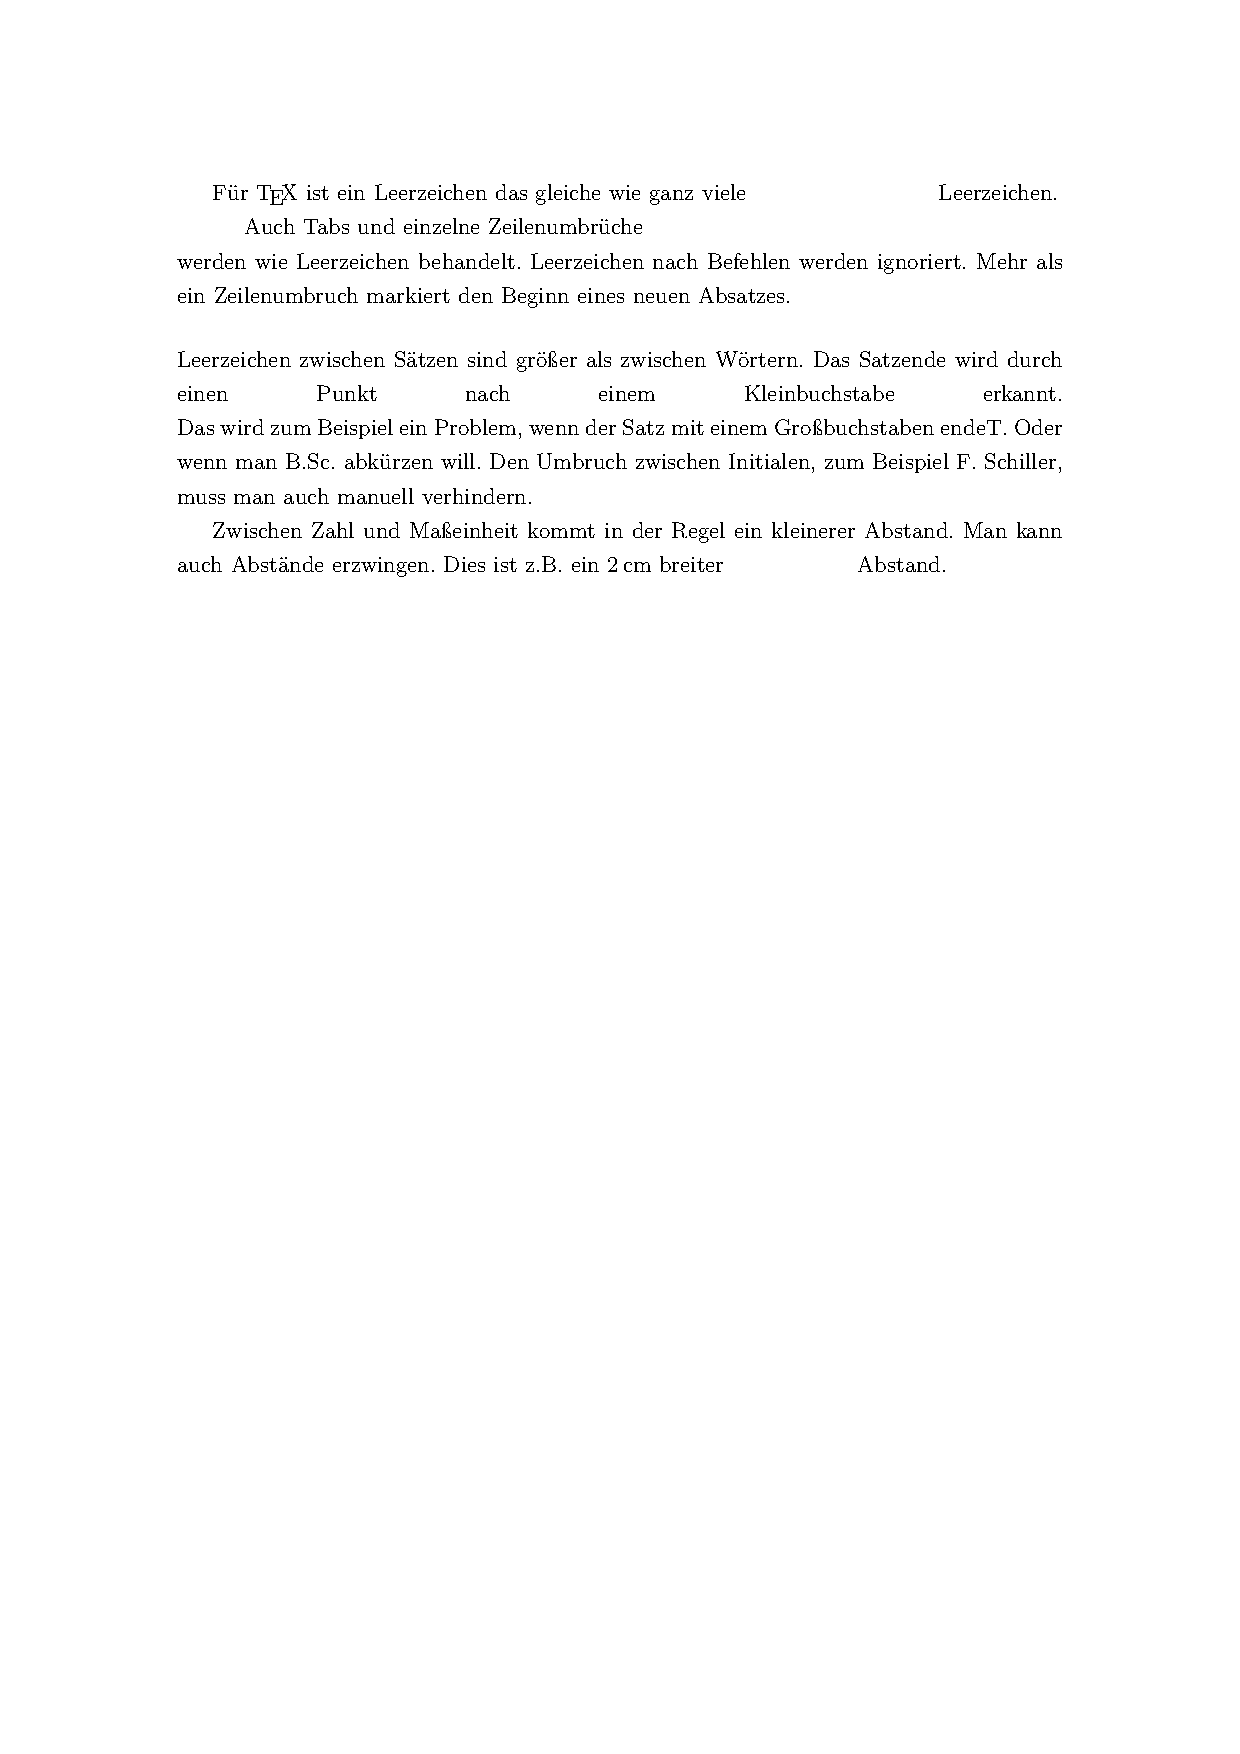
\includegraphics[width=\textwidth]{aufgabe13}

\noindent \underline{nachge\TeX t:}\\
\normalsize
%\begin{onehalfspacing}
\onehalfspacing
\indent Für \TeX \ ist ein Leerzeichen das gleiche wie ganz viele \hfill Leerzeichen.\\
\setlength{\parindent}{12mm} \indent 
Auch Tabs und einzelne Zeilenumbrüche\\
werden wie Leerzeichen behandelt. Leerzeichen nach Befehlen werden ignoriert.
Mehr als ein Zeilenumbruch markiert den Beginn eines neuen Absatzes.\\
\\
Leerzeichen zwischen Sätzen sind größer als zwischen Wörtern. Das Satzende wird durch\\
einen Punkt nach einem Kleinbuchstabe erkannt.\linebreak
Das wird zum Beispiel ein Problem, wenn der Satz mit einem Großbuchstaben endeT.\
Oder wenn man B.Sc.\ abkürzen will.
Den Umbruch zwischen Initialen, zum Beispiel F.~Schiller, muss man auch manuell verhindern.\\
\hspace*{4mm} Zwischen Zahl und Maßeinheit kommt in der Regel ein kleinerer Abstand.
Man kann auch Abstände erzwingen.
Dies ist z.B. ein 2cm breiter \hspace{2cm} Abstand.
%\end{onehalfspacing}

\pagebreak
\subsection{Listen}					% aufgabe 6
\begin{aufgabe}
\TeX en Sie folgenden Text so exakt wie m\"oglich nach.	
\end{aufgabe}

\noindent \underline{Ursprungstext:} \\
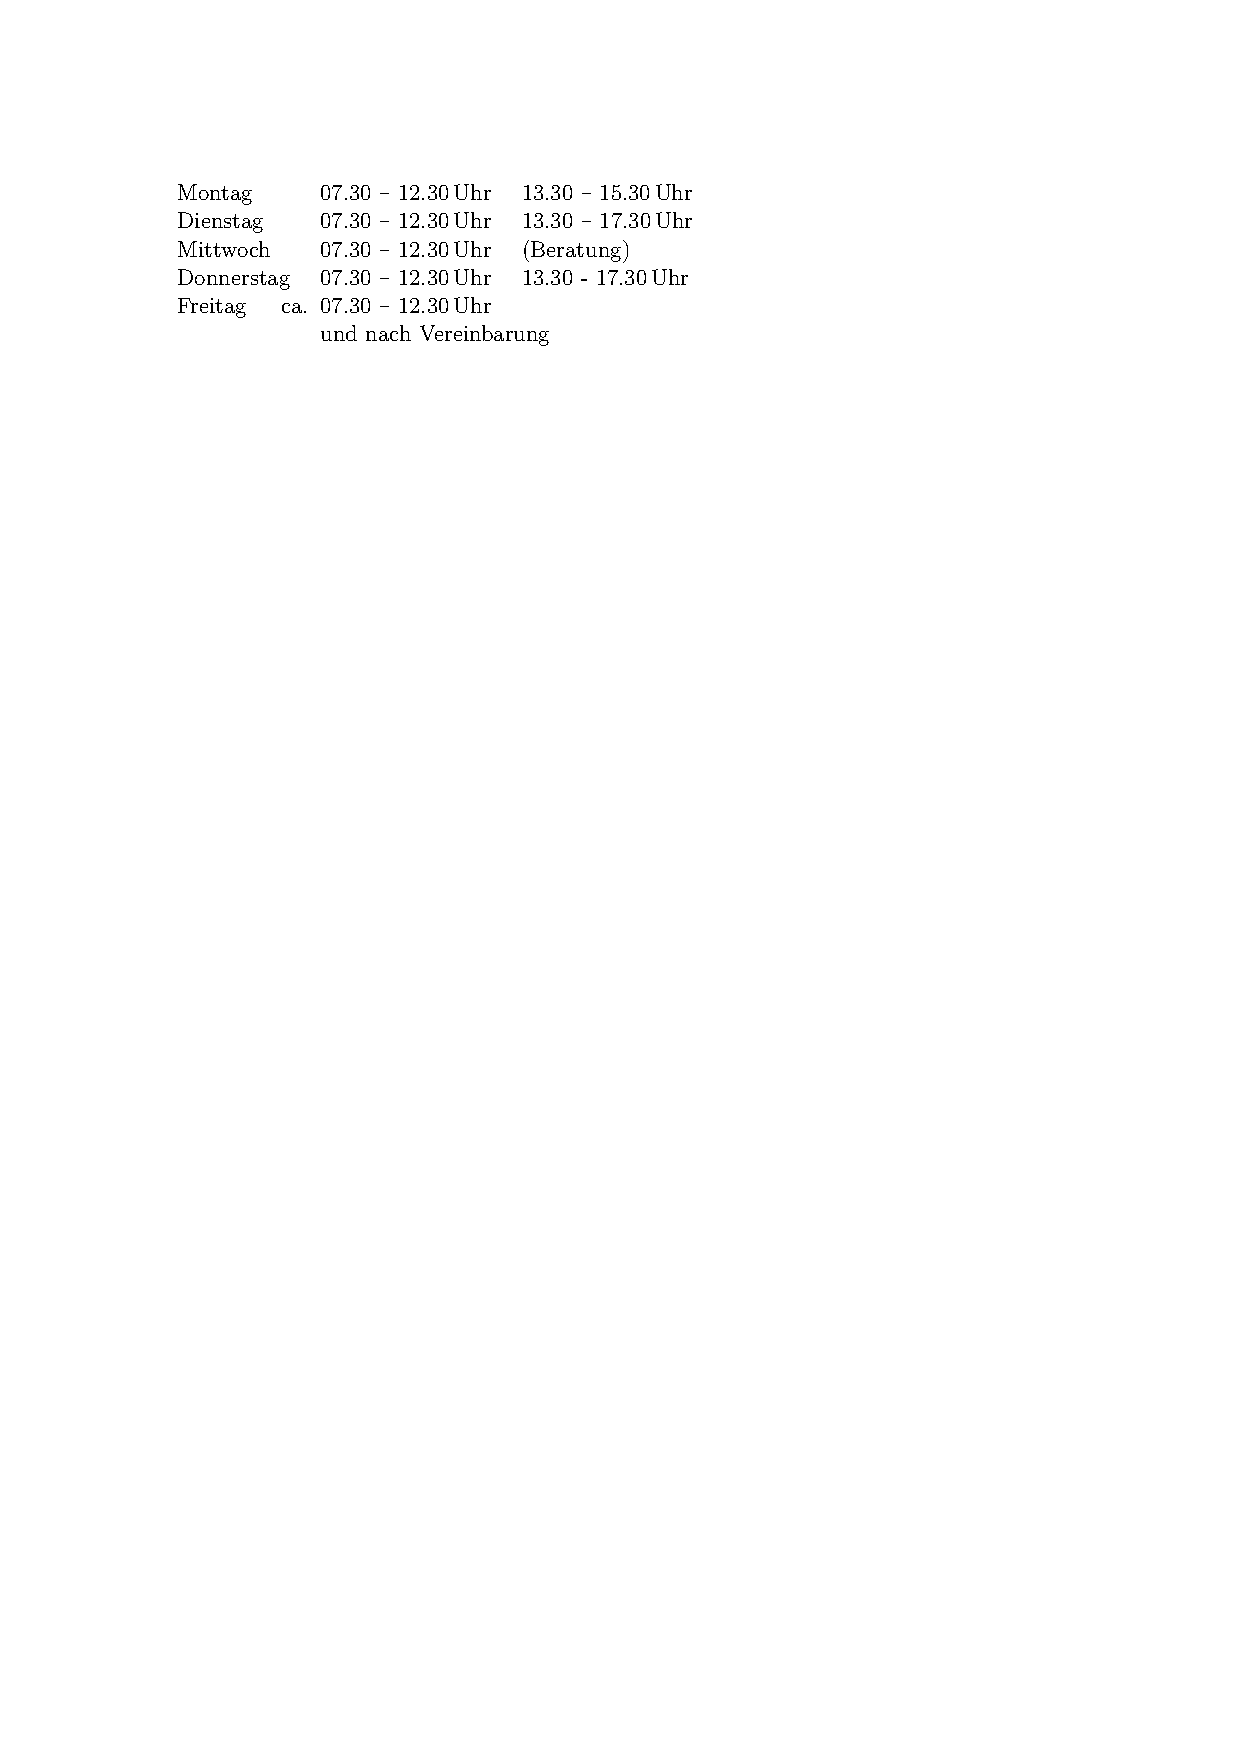
\includegraphics[width=\textwidth]{aufgabe14}

\noindent \underline{nachge\TeX t:}\\
\begin{singlespacing}
\hspace{-1.45cm}
\begin{tabular}{l l l}
Montag 		& 07.30 – 12.30 Uhr & \hspace{-0.9cm} 13.30 – 15.30 Uhr \\
Dienstag 	& 07.30 – 12.30 Uhr & \hspace{-0.9cm} 13.30 – 17.30 Uhr \\
Mittwoch 	& 07.30 – 12.30 Uhr & \hspace{-0.9cm} (Beratung) \\
Donnerstag 	& 07.30 – 12.30 Uhr & \hspace{-0.9cm} 13.30 – 17.30 Uhr \\
Freitag 	& \hspace{-0.74cm} ca. 07.30 – 12.30 Uhr &  \\
& und nach Vereinbarung & \\
\end{tabular}
\end{singlespacing}

\pagebreak
\begin{aufgabe}
Erstellen Sie folgende Liste.
\end{aufgabe}

\noindent \underline{Ursprungstext:} \\
\noindent
\includegraphics[width=\textwidth]{aufgabe15}

\noindent \underline{nachge\TeX t:}\\
Diese Unterlagen werden bei der Beantragung des Personalausweises benötigt:

\begin{itemize}
 \item[\ding{51}] gültiges Indentitätsbild
 \item[\ding{51}] aktuelles Lichtbild:
  \begin{itemize}
   \item[>] aktuelle Aufnahme
   \item[>] Frontalaufnahme, kein Halbprofil-Bild
   \item[>] das Gesicht muss zentriert auf dem Foto erkennbar sein
   \item[>] die Augen müssen offen und deutlich sichtbar sein
   \item[>] der Mund muss geschlossen sein und der Gesichtsausdruck neutral
  \end{itemize}
\end{itemize}


\begin{aufgabe}
Generieren Sie eine 1\,cm einger\"uckte Liste, die mit (A1), (A2), (A3),\dots\ gelabelt ist. Schreiben Sie darunter einen Satz, der auf das erste Element der Liste verweist.
\end{aufgabe}

\begin{enumerate}[\hspace{1cm} ({A}1)]
 \item Hund \label{it:hund}
 \item Katze \label{it:katze}
 \item Maus
 \item Marder
 \item Dachs
 \item Bieber
\end{enumerate}

\noindent Der Hund (A\ref{it:hund}) ist ein Haustier, das Geruch erzeugt.

\pagebreak
\begin{aufgabe}\label{aufg:desc}
Erstellen Sie eine \textnormal{\texttt{description}} Liste, in der Sie kurz
(je ein Satz) \TeX, \LaTeX\ und Word (im Hinblick auf deren Unterschiede)
beschreiben.
\end{aufgabe}

\begin{description}
 \item[\TeX] TeX ist ein Textsatzsystem mit eingebauter Makrosprache.
 \item[\LaTeX] LaTeX ist ist ein Softwarepaket, das die Benutzung des Textsatzsystems \TeX mit Hilfe von Makros vereinfacht.
 \item[Word] Word von Microsoft ist ein WYSIWYG-Editor.
\end{description}

\subsection{Fußnoten}						% aufgabe 6
\begin{aufgabe}
\label{aufg:18}
\setcounter{footnote}{2}
\renewcommand{\thefootnote}{\fnsymbol{footnote}}
F\"ugen Sie dieser Aufgabe eine Fu\ss note hinzu. Die Fu\ss{}note soll mit dem dritten Fu\ss{}notensymbol
gekennzeichnet sein. Sie soll mindestens 1\,cm  vom Haupttext entfernt mittels einer gepunkteten Linie 
abgetrennt werden.\footnote{Dies ist die Fußnote für Aufgabe \ref{aufg:18}.}
\end{aufgabe}

Vielleicht sollte aber auch die dritte Nummerierung benutzt werden. 
Schließlich steht ja nirgendwo festgeschrieben, 
dass~\verb*|\ddagger| das dritte Symbol ist. 
\hspace{-0.1cm}\footnote[3]{Dann ist das hier eine andere Fußnote für Aufgabe \ref{aufg:18}.}

\subsection{Randnotizen}
\begin{aufgabe}
Nutzen Sie Randnotizen um diese Aufgabe links mit einem 3\,mm breiten und 8\,mm hohen Balken zu markieren.

\reversemarginpar
\marginpar{\rule[0pt]{3mm}{8mm}}
\end{aufgabe}

\subsection{Boxen und Silbentrennung}
\begin{aufgabe}
\TeX en Sie folgende 3\,cm breite eingerahmte Box so exakt wie m\"oglich nach und achten Sie dabei insbesondere auf die korrekte Silbentrennung.
\end{aufgabe}

\noindent \underline{Ursprung:} \\
\noindent
\includegraphics[width=\textwidth]{aufgabe20}

\noindent \underline{nachge\TeX t:}\\
\indent \hspace{-0.7cm}
\fbox{\begin{minipage}{3cm}
  \begin{onehalfspacing}
   Gas\-chro\-ma\-to\-gra-\ \\phie\--Mass\-enspek-\ \\tro\-me\-trie
  \end{onehalfspacing}
\end{minipage}}

\subsection{Farben}						% aufgabe 6
\begin{aufgabe}
\"Andern Sie die Hintergrundfarbe nur dieser Seite in einen sehr hellen Pastellton (mindestens 90\,\% Wei\ss{}anteil). (Der Einfachheit halber k\"onnen Sie den n\"achsten Abschnitt auf einer neuen Seite beginnen.)
\end{aufgabe}
\pagecolor{LightGrey}